% !TeX program = pdfLaTeX
\documentclass[12pt]{article}
\usepackage{amsmath}
\usepackage{graphicx,psfrag,epsf}
\usepackage{enumerate}
\usepackage{natbib}
\usepackage{textcomp}
\usepackage[hyphens]{url} % not crucial - just used below for the URL
\usepackage{hyperref}
\providecommand{\tightlist}{%
  \setlength{\itemsep}{0pt}\setlength{\parskip}{0pt}}

%\pdfminorversion=4
% NOTE: To produce blinded version, replace "0" with "1" below.
\newcommand{\blind}{1}

% DON'T change margins - should be 1 inch all around.
\addtolength{\oddsidemargin}{-.5in}%
\addtolength{\evensidemargin}{-.5in}%
\addtolength{\textwidth}{1in}%
\addtolength{\textheight}{1.3in}%
\addtolength{\topmargin}{-.8in}%

%% load any required packages here



\usepackage{setspace}\doublespacing

\begin{document}


\def\spacingset#1{\renewcommand{\baselinestretch}%
{#1}\small\normalsize} \spacingset{1}


%%%%%%%%%%%%%%%%%%%%%%%%%%%%%%%%%%%%%%%%%%%%%%%%%%%%%%%%%%%%%%%%%%%%%%%%%%%%%%

\if0\blind
{
  \title{\bf Kaggle-in-class Data Challenges Can Boost Student Learning}

  \author{
        Julia Polak \\
    Department of Statistics, University of Melbourne\\
     and \\     Dianne Cook \\
    Department of Econometrics and Business Statistics, Monash University\\
      }
  \maketitle
} \fi

\if1\blind
{
  \bigskip
  \bigskip
  \bigskip
  \begin{center}
    {\LARGE\bf Kaggle-in-class Data Challenges Can Boost Student Learning}
  \end{center}
  \medskip
} \fi

\bigskip
\begin{abstract}
Kaggle is a data modeling competition service, where participants
compete to build a model with lower predictive error than other
participants. Several years ago they released a reduced service that
enables instructors to run competitions in a classroom setting. This
paper describes the results of an experiment to determine if
participating in a predictive modeling competition enhances learning.
The evidence suggests it does. In addition, students were surveyed to
examine if the competition improved engagement and interest in the
class.
\end{abstract}

\noindent%
{\it Keywords:} instructional technology, statistical modeling, data science, statistics education, data mining
\vfill

\newpage
\spacingset{1.45} % DON'T change the spacing!

\section{Introduction}\label{introduction}

Kaggle \citep{kaggle} is well-known for the data competitions, some
richly funded. It provides a platform for predictive modelling and
analytics competitions where participants compete to produce the best
predictive model for a given data set. In 2015, Kaggle InClass was
introduced, as a self-service platform to conduct competitions. These
competitions can be private, limited to members of a university course,
and are easy to setup. This paper examines the educational benefits of
conducting predictive modeling competitions in class on performance,
engagement and interest.

\section{Experimental setup}\label{experimental-setup}

\subsection{Data collection}\label{data-collection}

The experiment was conducted during Semester 2 2017. Data was collected
during two classes, one at the University of AB (MAST90083), and one at
CD University (ETC2420/5242).

\subsection{Competition data}\label{competition-data}

Two data sets were compiled for the kaggle challenges: Melbourne
property auction prices and spam classification. The Melbourne auction
price data was collected by extracting information from real estate
auction reports (pdf) collected between Feb 2, 2013 and Dec 17, 2016.
The spam classification data was compiled by graduate students at Iowa
State University as part of a data mining class, in 2009. Data was
compiled by monitoring and extracting information from their emails by
class members, over a period of a week, and manually tagging them as
spam or ham.

Both data sets were split into training and test sets, for the kaggle
challenge. Students had access to the true response variable only for
the training data. For the Melbourne housing data, students were
expected to predict price based on the property characteristics. For the
spam data, students were expected to build a classifier to predict
whether the email as spam or not.

Both data sets are challenging for prediction, with relatively high
error rates.

\subsection{Participants}\label{participants}

MAST90083 is titled Computational Statistics and Data Mining, is
designed for postgraduate level, for students with math, statistics,
information technology or actuarial backgrounds. It covers modelling
both continuous (regression) and categorical (classification) response
variables. The 63 students were randomized into one of two kaggle
competitions, one focused on regression (R) and the other classification
(C). Students built prediction models and made submissions individually
for 16 days, and then were allowed to form groups to compete for another
7 days.

ETC2420/5242, titled Statistical Thinking, covers regression, and has a
mix of undergraduate and postgraduate students. Only the 34 postgraduate
(5242) students were required to participate in the kaggle competition,
and competed in the regression (R) challenge. This was run independently
from the University of AB competition. The 145 undergraduate (2420)
students were used as controls for examining performance of the
postgraduate students. The competition ran for one month. Students
formed their own teams of 2-4 members to compete.

\section{Methodology}\label{methodology}

\subsection{Performance}\label{performance}

Better performance is equated to better understanding of the material,
as measured in the final exam. MAST90083 and ETC2420/5242 included
questions, with several parts, on the final exam related to kaggle
challenges. These questions were identified prior to data analysis.

For all questions in the exam, difficulty and discrimination scores were
computed, using the mean and standard deviations. Of the questions
pre-identified as being relevant to the data challenges, only the parts
that corresponded to high level of difficulty and high discrimination
were included in the comparison of performance.

Scores for the relevant questions were summed, and converted into
percentage of the possible score. The total exam score was converted to
a percentage. Performance for each student was computed as the ratio of
these two numbers. A value of 1 would indicate that the student's
performance on that set of questions was consistent with their overall
exam performance, greater than 1 that they performed better than
expected, and lower than 1 meant less than expected on that topic.

The distribution of the performance scores by group is shown as a
boxplot. Focus is on the difference in median between the groups.
Permutation tests were conducted to examine difference in median scores
for students participating or not in a competition.

\subsection{Engagement}\label{engagement}

The students were allowed to submit at most one prediction per day,
while the competitions were open. The frequency of submissions, and the
accuracy (or error) of their predictions, made by individual students,
is recorded as a part of the kaggle system. To examine whether
engagement improved performance, scores on the questions related to the
competition normalised by total exam score (as computed in the
performance section) is examined in relation to frequency of submissions
during the competition. In addition, performance in the competition as
measured by accuracy or error, is also examined in relation to the
number of submissions. Scatterplots, correlation and linear models are
used to examine the associations.

\subsection{Interest}\label{interest}

Students in MAST90083 and ETC5242 were invited to give feedback about
the course, in particular about the data competitions, before the final
exam. This information was voluntary, and students who completed the
questionnaire were rewarded with a coupon for a free coffee. The data
from this survey was viewed by the researchers after all course grades
had been reported.

\section{Results}\label{results}

\subsection{Performance}\label{performance-1}

Figure \ref{fig:MAST90083} shows the data collected in MAST90083.
Performance is plotted against type of question, separately for the
competition they completed. The difference in median scores indicates
performance improvement. Students who completed the classification
competition (left) performed relatively better on the classification
questions than the regression questions in the final exam. Conversely,
students who participated in the regression competition performed
relatively better on the regression questions.

\begin{figure}
\centering
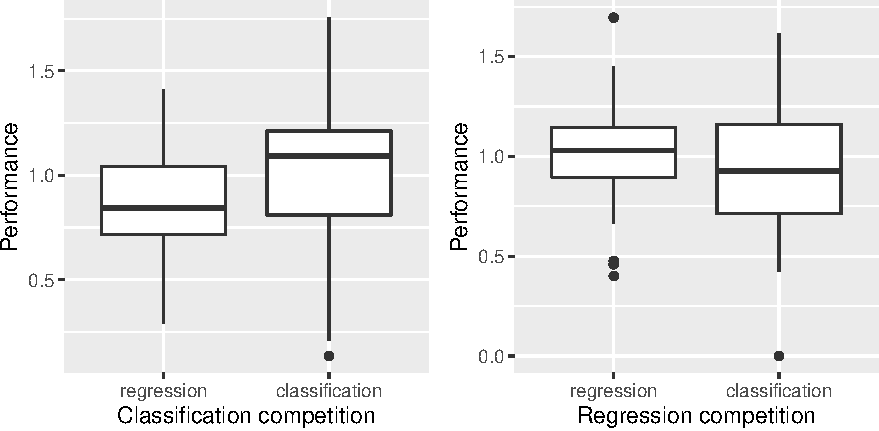
\includegraphics{paper-kaggle_files/figure-latex/Melb-1.pdf}
\caption{\label{fig:MAST90083} Boxplots of performance on regression and
classification questions in the final exam, by type of data competition
completed in MAST90083. Students generally performed better on the
questions corresponding to the competition they participated in.}
\end{figure}

\begin{table}[h]
\begin{center}
\begin{tabular}{|l|r|r|}\hline
Question Set & Median difference & Permutation $p$-value \\\hline
Classification & 0.250 & 0.033\\
Regression & 0.104 & 0.000\\\hline
\end{tabular}
\caption{Comparison of median difference in performance by competition group, for MAST90083 students, using permutation tests. Both sets of medians are significantly different, indicating improved scores for questions on the topic related to the Kaggle competition.}
\end{center}
\label{tab:Melb_Perm}
\end{table}

Table 1 shows the results of permutation testing of median difference
between the groups. Generally the results support the competition
improved performance. Students who participated in the kaggle challenge
for classification scored higher than those that did the regression
competition, on the classification problem. Using a permutation test,
this corresponds to a significant difference in medians. Similarly the
results show that students who did the regression challenge, performed
better on these exam questions.

Figure \ref{fig:ETC5242} shows the results for students ETC2420/5242.
The boxplots suggest that the students who participated in the challenge
performed relatively better than those that didn't on the regression
question than expected given their total exam performance.

Only the post-graduate students participated in the regression
competition, as their additional assessment requirement. Scores for the
question on regression (Q7a,b,c) in the final exam were compared with
the total exam score (RE). On these question parts, a, b, c, over all
the students all three were in the top 10 of difficulty, with students
scoring less than 70\%, on average. Parts b, c were in the top 10 for
discrimination, and part a was at rank 13.

\begin{figure}
\centering
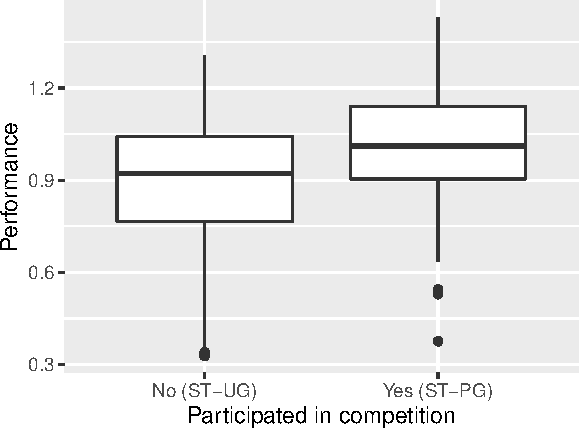
\includegraphics{paper-kaggle_files/figure-latex/ETC5242-1.pdf}
\caption{\label{fig:ETC5242} Performance for regression question
relative to total exam score for students who did and didn't do the
regression data competition in ETC2420/5242.}
\end{figure}

Based on the median, the students who participated in the kaggle
challenge scored 0.09 higher than those that didn't, a median of 1.01 in
comparison to 0.92. Using a permutation test, this corresponds to a
significant difference in medians, with \(p\)-value of 0.024.

\subsection{Engagement}\label{engagement-1}

The number of submissions that a student made, may be an indicator of
performance on the exam questions related to the competition. A student
who is more engaged in the competition may learn more about the
material, and consequently perform better on the exam. Figure
\ref{fig:numsubmition} (top row) shows performance on the classification
and regression questions, respectively, against their frequency of
prediction submissions for the three student groups (MAST90083
classification and regression, ETC5242 regression) competitions. The
relationship is weak in all groups, and this mirrors insignificant
results from a linear model fit to both subsets. On the other hand, the
predictive accuracy improved with the number of submissions for the
regression competitions.

The competition performance relative to number of submissions is shown
in plots (d)-(f). Each point corresponds to one student, and accuracy or
error of the best predictions submitted is used. The regression
competition seemed to engage students more than the classification
challenge. Students submitted more predictions, and their models
improved with more submissions.

\begin{figure}
\centering
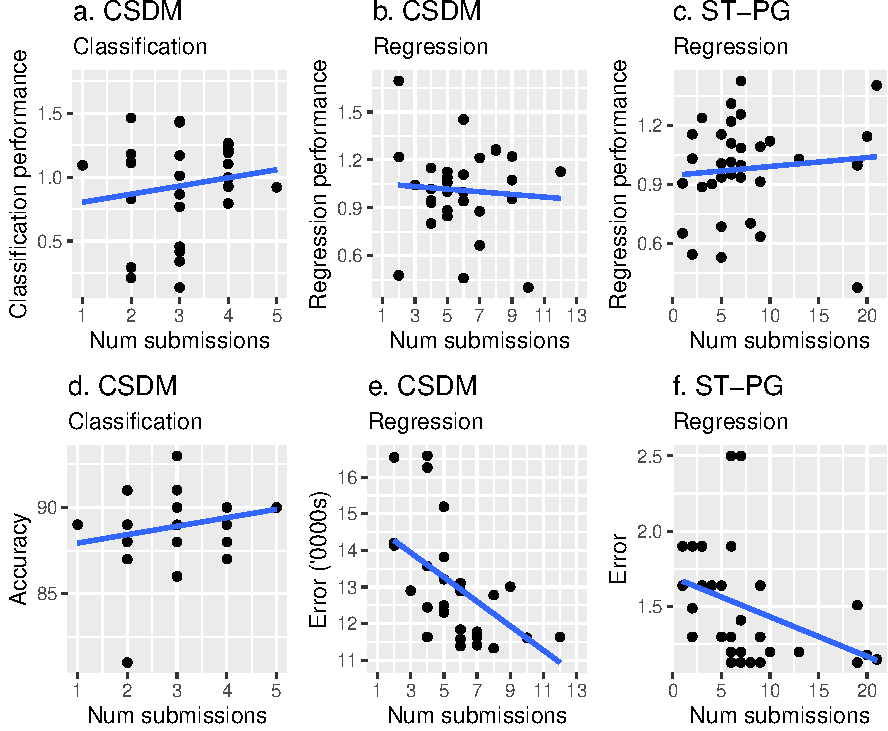
\includegraphics{paper-kaggle_files/figure-latex/numsubmition-1.pdf}
\caption{\label{fig:numsubmition} Scatterplots of the exam performance
(a-c) and competition performance (d-f) by number of prediction
submissions, for the three student groups. The relationships with exam
performance are weak. For the MAST90083 and ETC5242 regression
competitions, a clear pattern is that predictions improved substantially
with more submissions. (House price in ETC5242 were divided by 100,000,
explaining the difference in magnitude of error between two
competitions.)}
\end{figure}

\subsection{Interest}\label{interest-1}

Figure \ref{fig:likert} shows the survey responses related to the kaggle
competition, for MAST90083 and ETC5242. The response rate for MAST90083
was 55\%, with 34 of 61 students completed the survey. The response rate
for ETC5242 was 50\%, 17 students out of 34 completed the survey.
Overwhelmingly, students reported that they found the competition
interesting and helpful for their learning in the course.

\begin{figure}
\centering
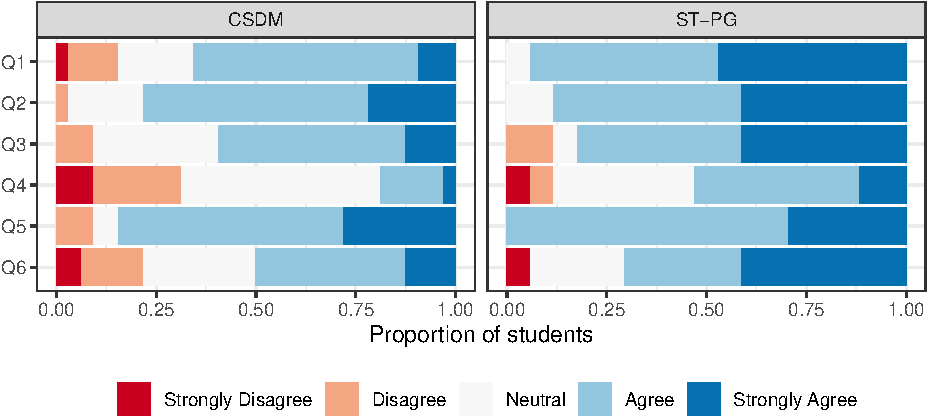
\includegraphics{paper-kaggle_files/figure-latex/likert-1.pdf}
\caption{\label{fig:likert}Summary of responses to survey of kaggle
competition participants. Overwhelmingly the response to the competition
was positive in both classes, especially the questions on enjoyment and
engagement in the class, and obtaining practical experience. (Table 2
lists the questions.)}
\end{figure}

\begin{table}[h]
\begin{center}
\begin{tabular}{|l|p{15cm}|}\hline
Label & Question \\\hline
Q1 & I found the data competition is great fun.\\\hline
Q2 & Taking part in the data competition contributed a lot to my engagement with the subject.\\\hline
Q3 & Taking part in the data competition improved my confidence in my understanding of the covered material.\\\hline
Q4 & Taking part in the data competition improved my confidence in my success in the final exam.\\\hline
Q5 & Taking part in the data competition improved my confidence in my ability to use the acquired knowledge in practical applications.\\\hline
Q6 & I feel that the required time investment in the data competition was worthy. \\\hline
\end{tabular}
\end{center}
\caption{Questions asked in the survey of competition participants.}
\label{survey_Q}
\end{table}

\section{Discussion}\label{discussion}

This paper has described the setup and results of an experiment to
examine the effectiveness of data competitions on student learning,
using Kaggle InClass as the vehicle for conducting the competition. The
experiment was conducted in the classroom settings as part of the normal
teaching of the courses, which imposes limitations on the design.
However, with both MAST90083 and ETC2420/5242, either a randomized
assignment of students to two topic groups, or a control group was
possible, which enabled comparing performance.

The primary finding is that participating in competitions results
produces a statistically significant improvement in the learning of the
topic, although the effect size is small. Secondarily, anecdotally, the
competitions enhanced interest and engagement in the course.

\section{Acknowledgments}\label{acknowledgments}

This project (title: Effect of Data Competition on Learning Experience)
has been approved by the Faculty of Science Human Ethics Advisory Group
University of AB (ID: 1749858.1 on September 4, 2017) and by CD
University Human Research Ethics Committee (ID: 9985 on August 24,
2017).

This document was produced in R \citep{R} with the package knitr
\citep{knitr}. Data cleaning was conducted using tidyr \citep{tidyr},
dplyr \citep{dplyr} and plots were made with ggplot2 \citep{ggplot2}.
The materials to reproduce the work are available at
\url{https://github.com/XXX}.

Information on setting up a Kaggle InClass challenge can be found at
\url{https://www.kaggle.com/about/inclass/overview}.

\bibliographystyle{agsm}
\bibliography{bibliography.bib}

\end{document}
